\documentclass[12pt]{report}
\usepackage{graphicx}
\usepackage{color}

\begin{document}

\chapter{Deep learning}
\begin{center}
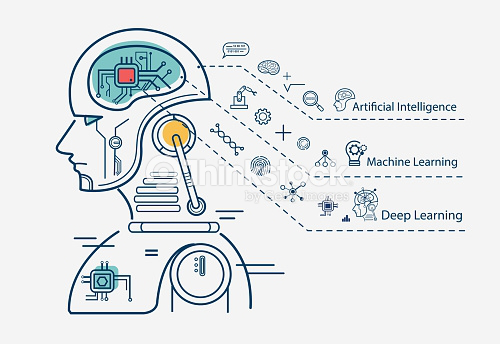
\includegraphics[width=300]{1.png} 
\end{center}

\newpage
\section{Introduction}
Au cours des dernières années, l'intelligence artificielle (IA) a fait l'objet d'un battage médiatique intense. L'apprentissage automatique, l'apprentissage en profondeur et l'IA apparaissent dans d'innombrables articles, souvent en dehors des publications axées sur la technologie .Alors abordons ces questions: qu'a-t-on appris jusqu'à présent l'apprentissage profondeur? Quelle est son importance? Où nous allons ensuite?
\\
  l'apprentissage en profondeur est un progrès relativement récent dans la programmation de réseaux de neuronaux, l'apprentissage en profondeur est composé d'un certain nombre de technologies différentes \cite{ref10} .\\
  Ce chapitre vous donnera une compréhension fondamentale de ce qu'est l'apprentissage en profondeur, de ce qu'il peut accomplir et de son fonctionnement, Cela vous familiarisera également avec le processus canonique de résolution de problèmes de données utilisant un apprentissage approfondi \cite{ref10} . 
    \\
  ce chapitre comporte la notion d'apprentissage automatique et ça puissance avec les méthodes et les technique utilisé par l'apprentissage profondeur      
 et les différentes algorithmes aussi les types de modelés de prédiction tel que la régression  et classification \cite{ref10} .

\newpage
\section{L'apprentissage automatique}

\subsection{Introduction}

L'apprentissage automatique est un sous-domaine de l'intelligence artificielle(IA). En général, l'objectif de l'apprentissage automatique est de comprendre la structure des données et de les intégrés dans des modèles qui peuvent être compris et utilisés par tout le monde \cite{ref10}.
 Les algorithmes d'apprentissage automatique permettant aux ordinateurs de s'entraîner sur les entrées de données et utilisent l'analyse statistique pour produire des valeurs qui se situent dans une plage spécifique. Pour cette raison, l'apprentissage automatique facilite l'utilisation des ordinateurs dans la construction de modèles à partir de données d'échantillonnage afin d'automatiser les processus de prise de décision en fonction des données saisies.

\subsection{Définition}
l'apprentissage automatique en anglais machine learning,ou l'apprentissage statique est un champ d'étude de l'intelligence artificielle qui se fonde sur des approches statistiques pour donner aux ordinateurs la capacité d'apprendre à partir de données, c'est-à-dire d'améliorer leurs performances à résoudre des tâches sans être explicitement programmés pour chacune.\\ Plus largement, cela concerne la conception, l'analyse, le développement et l'implémentation de telles méthodes \cite{ref11} .

\subsection{Différentes méthodes d'apprentissage automatique}
  \subsubsection{Apprentissage supervisé}
utilisé certaines variable pour prédire des valeurs inconnues au future d'autres variables par rapport la variable cible se base en deux modèle la régression et la classification. Dans la section suivante, nous allons nous intéresser plus particulièrement à la régression \cite{ref11} .



\subsubsection{Apprentissage non supervisé}
Trouver des formes interprétables par un humain permettant de décrire les données sans utiliser de variables cible à prédire \cite{...} .
\\
 le clustering est parmi l'apprentissage non supervisé qui basent sur une mesure de similarité, est généralement mesurée en termes de distances \cite{ref11} .


\subsubsection{Apprentissage semi supervisé}
Effectué de manière probabiliste ou non, il vise à faire apparaitre la distribution sous-jacente dans leur espace de description. Il est mis en œuvre quand des données manquent,Le modèle doit utiliser des exemples non étiquetés pouvant néanmoins renseigner \cite{ref11} .
\subsubsection{Différence entre l'apprentissage supervisé et non supervisé }
l'apprentissage non supervisé + label = l'apprentissage supervisé.\\

\begin{figure}[h]
\begin{center}
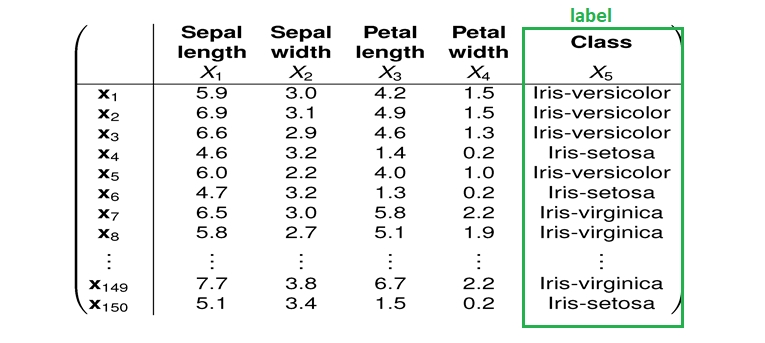
\includegraphics[width=300]{iris.jpg} 
\caption{Data Iris}
\label{Data Iris}
\end{center}

\end{figure}

aussi l'apprentissage supervisé basé sur la notion de train Data on prend par exemple sur l'ensemble des données Iris data \cite{ref11} .


\subsubsection{Prédiction}
La prédiction consiste à estimer la valeur d'une variable continue dit cible ou dépendante.  La variable cible peut représenter :
\begin{enumerate}
\item la classe à laquelle appartient chaque point de données ou
\item Un attribut mesurable 
\end{enumerate}

\subsection{Modèle prédictif et modèle descriptif}
Un modèle prédictif suppose la présence d'une variable cible alors qu'un modèle descriptif n'en suppose aucune.\\
Dans un modèle prédictif, l'analyse est guidée par la variable cible \cite{ref11}. 

\section{prédiction du variable cible}
Deux façons de faire selon le type de la variable cible :
\begin{enumerate}
\item \textbf{Régression}
\item \textbf{Classification} 

\end{enumerate}

\subsection{Modèle de régression}

\subsubsection{Définition}
Une méthode statistique qui permet d'étudier le type de relation pouvant exister entre une certaine variable (dépendante) dont on veut expliquer les valeurs et une ou plusieurs autres variables explicatives qui servent à cette explication (variables indépendantes) \cite{ref11} . \\
Le modèle de régression est un modèle prédictif qui permet d'expliquer une variable cible quantitative par une ou plusieurs variables explicatives quantitatives.





\begin{enumerate}
\item Régression linéaire simple

\item Régression linéaire multiple

\item Régression non linéaire
\end{enumerate}


\subsubsection{Régression linéaire simple}
dite simple si elle permet de prédire les valeurs d’une variable cible (expliquée (Y)) à partir des valeurs prises par une autre variable dite (explicative (X)) \cite{ref11} . \\
Ainsi, une régression linéaire simple va permettre de résumer, d’interpréter et de prévoir les variations d’une variable dépendante (Y) en fonction d’une autre variable dite indépendante (X) et ce en utilisant une droite.

\subsubsection{Régression linéaire multiple}
dite multiple si elle permet de prédire les valeurs d’une variable cible(expliquée (Y)) à partir des valeurs prises par plusieurs autres variables dites indépendantes (explicatives (Xi)) \cite{ref11}.
\subsubsection{Régression non linéaire}
La régression non linéaire est une méthode permettant de déterminer un modèle non linéaire de relation entre la variable la variable cible et un groupe de variables indépendantes (explicatives (Xi)).a l'inverse de la régression linéaire classique, qui se limite aux modèles linéaires de prévision, la régression non linéaire peut élaborer des modèles avec des relations arbitraires entre variables dépendantes et indépendantes.
\begin{figure}[h]
\begin{center}
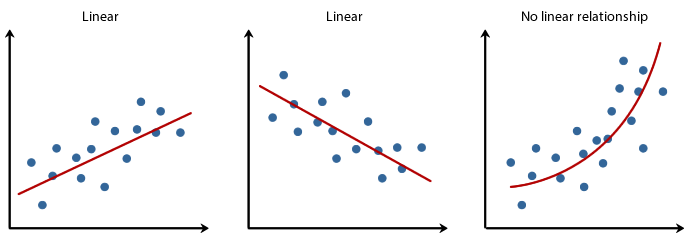
\includegraphics[width=300]{rg.png}
\end{center}
\caption{}
\label{}
\end{figure}




\subsection{Modèle de classification}
\subsubsection{Définition}
La classification supervisée permet de prédire si un élément est membre d’un groupe ou d’une catégorie donnée. 

\subsection{Classement et Classification }
Le \textbf{Classement} consiste à placer chaque individu dans une classe, parmi plusieurs classes prédéfinies en fonction des caractéristiques.\\\\
La \textbf{classification} consiste à regrouper les individus d'une population en un nombre limité de classes qui ne sont pas prédéfinies mais déterminées au cours de l'opération.

\subsection{Techniques de classification}

\begin{enumerate}
\item Arbres de décision
\item k-Plus Proches Voisins
\item Réseaux de neurones
\item Support Vector Machines
\end{enumerate}

\subsection{Arbre de décision}
Un modèle prédictif permettant d'obtenir par induction des conclusions plus générales à partir de faits particuliers.\\\\

\begin{figure}[h]
\begin{center}
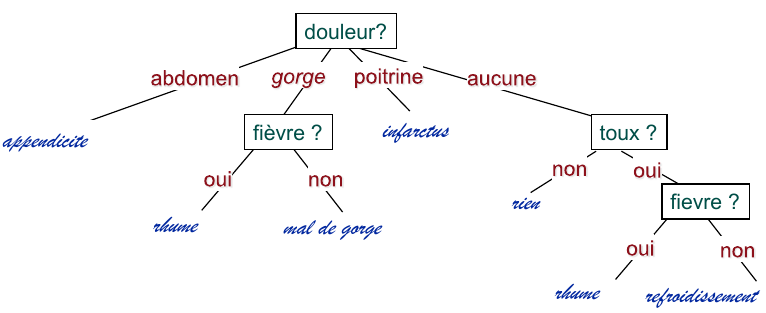
\includegraphics[width=400]{add2.png}
\caption{Arber de décision}
\label{}
\end{center}


\end{figure}

\newpage
\subsection{Structure d'un arbre de décision}
\begin{enumerate}
\item Chaque noeud interne correspond à un attribut.
\item Chaque branche correspond à valeur possible de cet attribut.
\item Chaque feuille correspond à une classe et fournit une classification.
\item Chaque chemin dans l'arbre correspond à une règle.

\end{enumerate}

\subsection{K-Plus Proches Voisins( KNN )}
C'est une méthode de classification supervisée  basée sur l'analogie.\\
C'est une des méthodes de classification les plus simples.\\\\

\begin{figure}[h]
\begin{center}
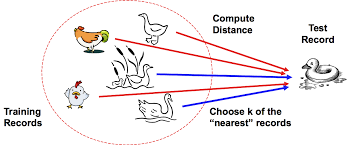
\includegraphics[width=400]{knn.png}
\caption{K-plus proches voisin}
\label{K-plus proches voisin}
\end{center}
\end{figure}
\\\\
Choix de la distance par attribut et du mode de combinaison des distances.






%la partie 2eme consernent le Deep learning trée important

\newpage
\section{Deep learning}

\subsection{Définition}
 est un ensemble des méthodes d’apprentissage automatique tentant de modéliser avec un haut niveau d’abstraction des données grâce à des architectures articulées de différentes transformations fondées sur l’apprentissage de modèles de données. Une observation (une image, p. ex.) peut être représentée de différentes façons par un vecteur de données.

\subsection{pour quoi l'utilisation de Deep learning}
Les deux idées clés de l'apprentissage en profondeur pour la vision par ordinateur - réseaux de neurones convolutionnels et rétropropagation - étaient déjà bien comprises en 1989. L'algorithme LSTM (Long Short Term Memory), fondamental pour un apprentissage en profondeur pour la série temporelle, a été développé en 1997.
 et a à peine changé depuis. Alors pourquoi l'apprentissage en profondeur n'a-t-il démarré qu'après 2012? Qu'est-ce qui a changé dans ces deux décennies?
En général, trois forces techniques sont à l'origine des progrès de l'apprentissage automatique:
\begin{enumerate}
\item  matériel
\item  Jeux de données
\item l'avancement d'algorithmiques
\end{enumerate}
\\
Les algorithme de machine learning n’est pas efficace pour les données volumineuses,Le deep learning est capable de traiter les données volumineuses.\\
dans le deep learning, on utilise un réseau de neurones artificiels qui a pour but d'apprendre seul à résoudre le problème, à l'aide d'une ensemble de données.

\subsection{La démocratisation de l'apprentissage profondeur}
La démocratisation des outils utilisés sur le terrain est l’un des facteurs clés de cet afflux de nouveaux visages dans l'apprentissage en profondeur \cite{ref12} . À ses débuts, l'apprentissage en profondeur nécessitait une expertise considérable en C ++ et CUDA, que peu de gens possédaient. De nos jours, les compétences de base en scripts Python suffisent pour effectuer des recherches approfondies en profondeur. Cela s’explique notamment par le développement de Theano, puis de TensorFlow, deux frameworks symboliques de manipulation tenseur pour Python prenant en charge l'autodifférenciation, simplifiant grandement la mise en œuvre de nouveaux modèles, et par la montée en puissance de bibliothèques conviviales telles que Keras, ce qui rend l'apprentissage en profondeur aussi facile que la manipulation de briques LEGO. Après sa sortie au début de 2015, Keras est rapidement devenu la solution d'apprentissage en profondeur par excellence pour un grand nombre de nouvelles entreprises en démarrage, d'étudiants diplômés et de chercheurs sur le terrain.

\subsection{Les réseaux de neurones artificiel (ANNs)}
Un réseau de neurone artificiel, ou réseau neuronal artificiel, est un système dont la conception est à l'origine schématiquement inspirée du fonctionnement des neurones biologiques, et qui par la suite s'est rapproché des méthodes statistiques \cite{ref12} .\\
\begin{figure}[h]
\begin{center}
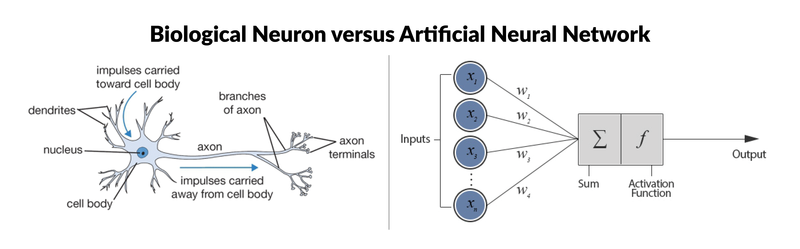
\includegraphics[width=450]{bio.png}
\caption{réseau neuronal}

\end{center}
\end{figure}


utiliser pour extraire des règles et des tendances à partir de données compliquées, bruitées et imprécises. Ils peuvent s'utiliser pour extraire des modèles et détecter des tendances reposant sur des fonctions mathématiques compliquées qui sont trop difficiles, voire impossible, à modéliser à l'aide de techniques analytiques ou paramétriques traditionnelles \cite{ref12} .
\subsection{Les taches des réseaux de neurones (ANNs) }
les réseaux de neurones sont en mesure d'effectuer différentes catégories de tâches, notamment de la \textbf{régression} et de la \textbf{classification}, Les tâches de régression visent à mettre en relation un certain nombre de variables d'entrée x avec un ensemble de résultats continus t (les variables cible). Par opposition, les tâches de classification visent à affecter des observations aux classes d'une variable cible catégorielle en fonction d'un ensemble de valeurs d'entrée \cite{ref13} .

\subsection{Utilisation des Réseaux de Neurones}
Les réseaux de neurones ont une remarquable faculté à donner un sens, extraire des règles et des tendances à partir de données compliquées, bruitées et imprécises. Ils peuvent s'utiliser pour extraire des modèles et détecter des tendances reposant sur des fonctions mathématiques compliquées qui sont trop difficiles, voire impossible, à modéliser à l'aide de techniques analytiques ou paramétriques traditionnelles \cite{ref13} .  les réseaux de neurones sont particulièrement bien adaptés à l'application de problématiques concrètes dans les domaines de la recherche scientifique, un certain nombre de domaines dans lesquels les réseaux de neurones ont été appliqués avec succès :

\begin{enumerate}
\item Robotique
\item Classification
\item Analyse de l'image et synthèse vocale
\item Diagnostiques et suivi médical

\end{enumerate}
 



\subsection{Les réseaux de neurones convolutif (CNN)}
Le réseau de neurones convolution (CNN) est une technologie de réseau de neurones qui a eu un impact profond sur le domaine de la vision par ordinateur (VC).Fukushima en 1980 a introduit le concept original d'un réseau de neurones convolutionnel. \\
la convolution est une technologie importante souvent combiné avec l'apprentissage profondeur \cite{ref13} . Hinton en 2014 a introduit la convolution pour permettre aux réseaux de reconnaissance d'images de fonctionner de la même manière que les systèmes biologiques et d'obtenir des résultats plus précis \cite{ref13} .\\
\newpage
\subsection{Définition}
réseaux d'unités de calcul élémentaire inter connectées,algorithmes pour résoudre des problèmes complexes.Le réseau de neurones artificiels est un moyen de modélisation du mécanisme d'apprentissage et de traitement de l'information qui se produit dans le cerveau humain afin de reproduire certaines caractéristiques \cite{ref13}   .\\
Déterminer un réseau de neurones = Trouver les coefficients synaptiques.\\
On parle de phase d'apprentissage : les caractéristiques du réseau sont modifiées jusqu'à ce que le comportement désiré soit obtenu.

\subsection{Structure de base de CNN}
Une conception typique de CNN commence par l'extraction des caractéristiques et se termine par la classification. L'extraction des caractéristiques est effectuée en alternant des couches de convolution avec des couches de sous-échantillonnage. La classification est effectuée avec des couches denses suivies d'une couche finale softmax. Pour la classification des images, cette architecture fonctionne mieux qu'un réseau de neurones à rétroaction intégrale entièrement connecté \cite{ref13} .
\begin{figure}[h]
\begin{center}
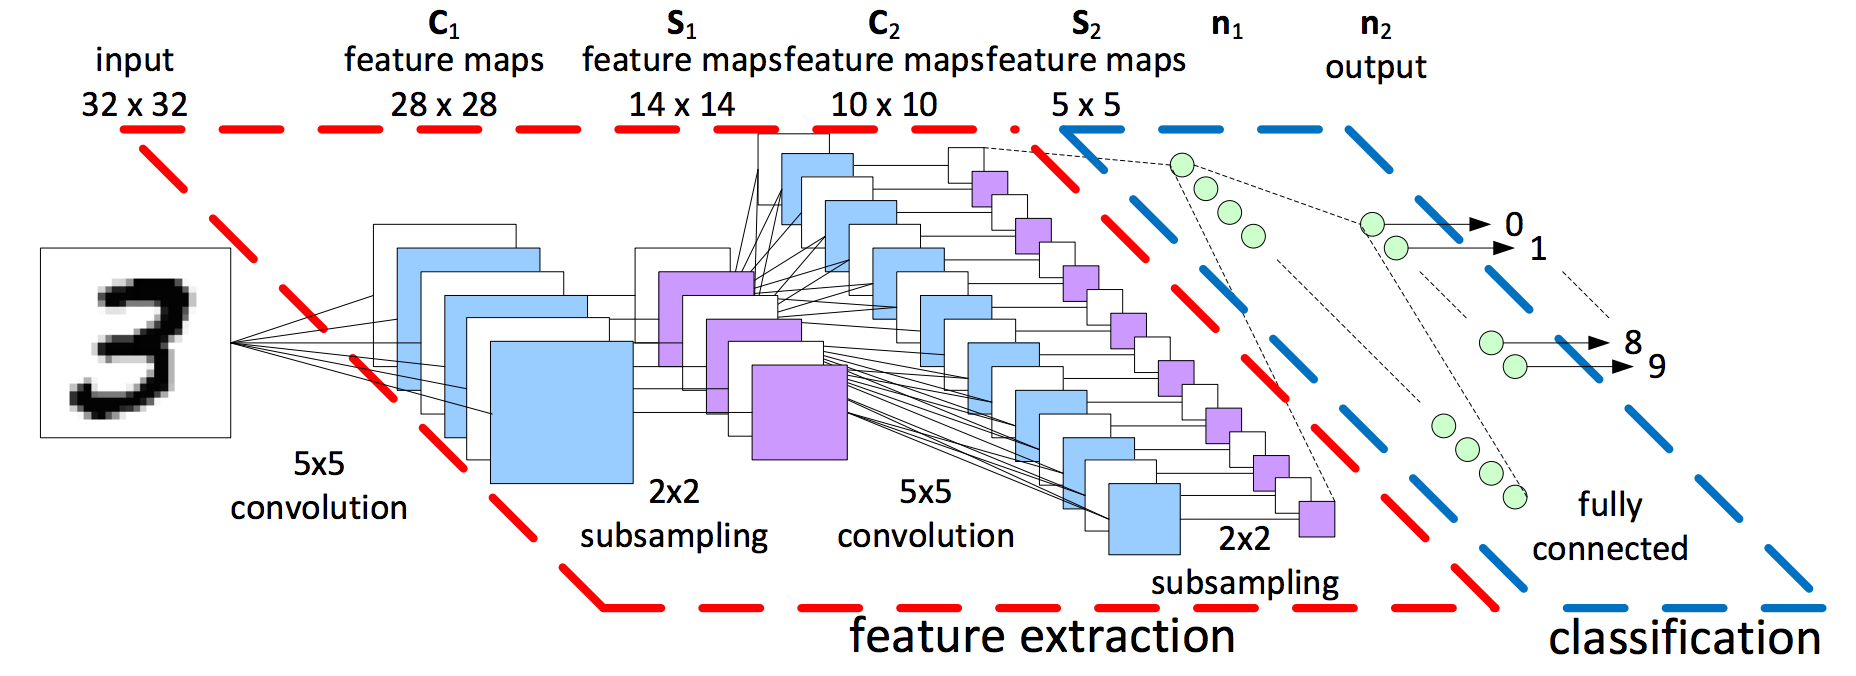
\includegraphics[width=300]{extract.png}
\caption{Structure de CNN}
\label{Structure de CNN}
\end{center}
\end{figure}


\subsection{Les Couches utilisées pour construire des CNN}
Comme nous l'avons décrit ci-dessus, un ConvNet simple est une séquence de couches et chaque couche d'un ConvNet transforme un volume d'activations en un autre à l'aide d'une fonction différentiable. Nous utilisons trois types principaux de couches pour construire des architectures ConvNet: la couche convolutionnelle, la couche de regroupement et la couche entièrement connectée (exactement comme dans les réseaux de neurones normaux). Nous allons empiler ces couches pour former une architecture ConvNet complète \cite{ref14}.
\begin{figure}[h]
\begin{center}
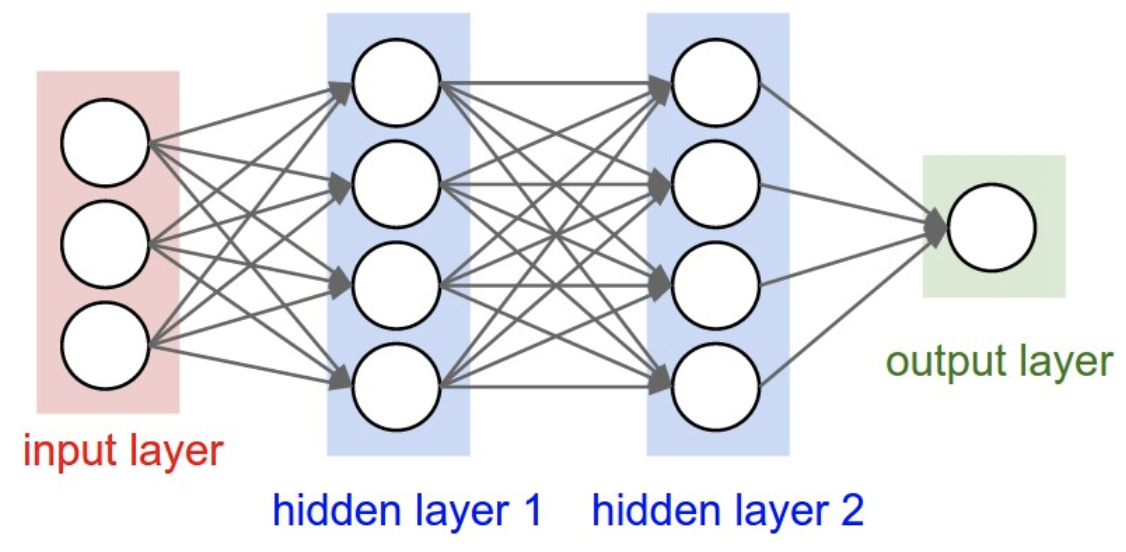
\includegraphics[width=300]{nnda.png}
\caption{Les couches de CNN}
\label{Les couches de CNN}
\end{center}
\end{figure}



\subsection{Caractéristiques et avantages CNN}
Un avantage majeur des réseaux convolutifs est l'utilisation d'un poids unique associé aux signaux entrant dans tous les neurones d'un même noyau de convolution.Cette méthode réduit l'empreinte mémoire, améliore les performances et permet une invariance du traitement par translation \cite{ref14}.\\
C'est le principal avantage du réseau de neurones convolutifs par rapport au perceptron multicouche, qui lui considère chaque neurone indépendant et affecte donc un poids différent à chaque signal entrant.

\subsection{Architecture de CNN}
Plusieurs architectures dans le domaine des réseaux de convolution Les plus courants sont:
\subsubsection{LeNet}
Les premières applications réussies de réseaux de convolution ont été développées par Yann LeCun dans les années 1990. Parmi celles-ci, la plus connue est l'architecture LeNet utilisée pour lire les codes postaux, les chiffres, etc \cite{ref15} .
\subsubsection{AlexNet}
Le premier travail qui a popularisé les réseaux de convolution dans la vision par ordinateur a été AlexNet, développé par Alex Krizhevsky, Ilya Sutskever et Geoff Hinton  .
\subsubsection{GoogLeNet}
ILSVRC 2014 était un réseau de convolution de de Google, Sa principale contribution a été la mise au point d'un module de démarrage réduisant considérablement le nombre de paramètres dans le réseau (4 M, par rapport à AlexNet avec 60 M) \cite{ref15}.



\subsection{LeNET-5}
LeNET-5 est une architecture primaire du classification pour l'images graphiques, le réseau LeNET-5 contient plusieurs types de couche diffirent et données flux de l'entrée à la sortie.
\begin{figure}[h]
\begin{center}
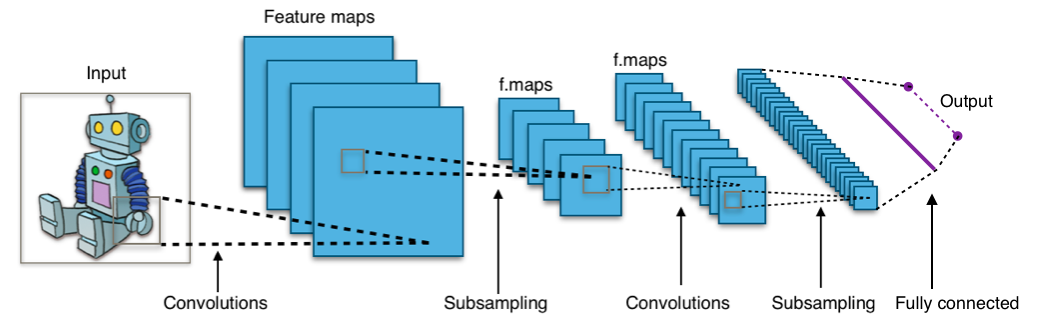
\includegraphics[width=400]{cnn.png}
\caption{LeNET-5}

\end{center}
\end{figure}
\\
Dans le cadre de la reconnaissance d'image, cette dernière est ( pavée ), c'est-à-dire découpée en petites zones (appelées tuiles). Chaque tuile sera traitée individuellement par un neurone artificiel (qui effectue une opération de filtrage classique en associant un poids à chaque pixel de la tuile) \cite{ref15}.



\newpage
\subsection{Ensembles d'apprentissage et d'évaluation}
Un\textbf{ ensemble d'évaluation }est un ensemble de données utilisé pour évaluer le modèle développé à partir d'un ensemble d'apprentissage \cite{ref15} .% par google
\\
par exemple,nous avons obtenu énormément de données nous pouvont diviser l'ensemble de données en deux partie,avec un ensemble  sera grand que l'autre puis en utiliser la partie grande pour l'apprentissage et l'autre pour l'évaluation \cite{ref15} .

\subsection{Données de qualité}
Évidemment, si vos données d'entraînement sont pleines d'erreurs, de valeurs aberrantes et de bruits (en raison de mesures de mauvaise qualité, par exemple), il sera plus difficile pour le système de détecter les modèles sous-jacents. Par conséquent, votre système sera moins performant. Cela vaut souvent la peine de passer du temps à nettoyer vos données de formation. En réalité, la plupart des scientifiques de données consacrent une grande partie de leur temps à cela  \cite{ref16}.

\subsection{Entraînement et Validation}
La création d'un ensemble d'apprentissage et d'un ensemble d'évaluation à partir d'un ensemble de données vous permet de déterminer si un modèle spécifique généralisera bien les nouvelles données \cite{ref15} .\\
\begin{figure}[h]
\begin{center}
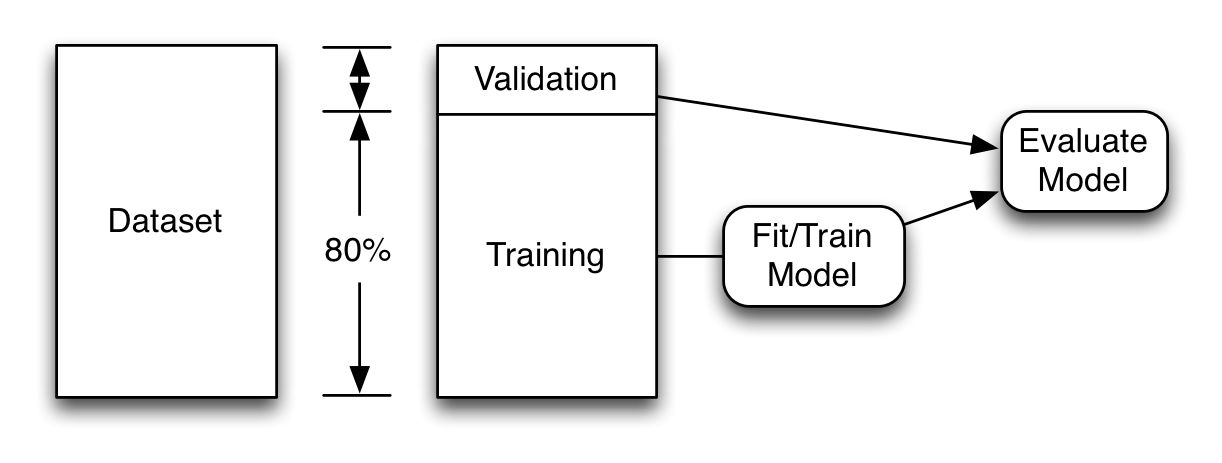
\includegraphics[width=300]{evalu.png}
\caption{Entrainement et Validation}

\end{center}

\end{figure}


 Il existe deux moyens principaux de traiter les données de formation et de validation:
\subsubsection{Entraînement/validation split}
Les données sont réparties selon un certain rapport entre un ensemble de évaluation et de validation. Les ratios habituels sont \textbf{80/100}  pour entrainement formation et \textbf{20/100}  pour validation  \cite{ref16}.

\subsubsection{K-Fold Cross Validation}
Les données sont divisées en un certain nombre de plis et de modèles. Étant donné qu'un nombre de modèles égal aux plis est créé, des prédictions hors échantillon peuvent être générées pour l'ensemble du jeu de données  \cite{ref17}.

\subsection{Représentation}
Un modèle de Machine Learning ne peut pas directement voir, entendre ou sentir les exemples d'entrée. Vous devez donc créer
une\textbf{ représentation }des données pour fournir au modèle un angle de vue utile sur les qualités clés des données. Autrement dit, pour entraîner un modèle, vous devez choisir l'ensemble de caractéristiques qui représentent le mieux les données.\\
Certaines représentations et une bonne capacité d’analyse automatique des différenciations rendent la tache d'apprentissage plus efficace.




\newpage
\section{Conclusion}
Les systèmes d'apprentissage en profondeur représente ensemble des tache qui amélioré la précision avec des outils très puissant qui permet d'effectuer de multiples actions encore de créer un programme évolutionnaire qui s'améliore sans cesse. Le présent document est centré sur la manière dont l'apprentissage en ensemble peut être appliqué à ces différents systèmes d'apprentissage en profondeur pour obtenir une plus grande précision de reconnaissance \cite{ref17}.\\
les réseaux de neurones convolutionnels est un domaine très actif dans le domaine de la vision par ordinateur.

\newpage
\bibliographystyle{plain}
\bibliography{biblioDeep}

\end{document}



